\section{Xアームの基線長伸縮スペクトル}
基線長伸縮は、共振器制御にとって、制御信号に乗るので小さく低減されるのが望ましい。とくにRMSが大きい脈動は、制御を不安定にする主な原因となっており、それを低減するための工夫を必要とする。一つの簡単な方法は、共振器をブレッドボードに乗せることである。これにより2つの鏡同士は相関をもち、とくに脈動のような低周波地面振動では同相で鏡が動くため、逆相成分が同相成分と比べて相対的に低減される。この考えに立つと、KAGRAの腕共振器も飛騨片麻岩の上に固定しており、ある程度相関をもっていると思われる。本章では、どの程度Xアームで逆相成分が低減されているか評価することにした。


\subsection{同相成分と逆相成分}
2点での変位$x_{1}$と$x_{2}$について,これら2つの同相成分$x_{\mathrm{com}}$と逆相成分$x_\mathrm{diff}$を
\begin{eqnarray}\label{eq:eq22}
  x_{\mathrm{diff}} &\equiv& \frac{x_{1}-x_{2}}{\sqrt{2}}, \\
  x_{\mathrm{com}}  &\equiv& \frac{x_{1}+x_{2}}{\sqrt{2}}
\end{eqnarray}
と定義する。パワーが保存するように、規格化定数は$\sqrt{2}$にしている。


同相成分は重心移動をあらわし,逆相成分は伸縮を表す。

\subsection{Common Differential Mode Rate (CDMR)}
2点が相関をもって動く場合,同相成分と逆相成分の比は1:1にはならない。たとえば0.2Hzの脈動の波長は,弾性波の速度を$5500\, \mathrm{m/s}$とすると,$10\,\mathrm{km} $となるので,数mスケールではほとんど一体となって地面は揺れ,2点は同相でうごき,逆相成分は相対的に小さくなる。共振器長制御をするうえで,基線長伸縮である逆相成分を小さく低減することが望ましい。基線長伸縮がどの程度低減されているかを表す指標として,同相成分と逆相成分のパワー比を以下で定義する。


2つの信号の同相成分と逆相成分の比、Common Differential Mode Rate (CDMR) を
\begin{equation}
  \boxed{\mathrm{CDMR} \equiv \sqrt{\frac{同相成分のパワー}{逆相成分のパワー}} = \sqrt{\frac{P_{\mathrm{com}}(\omega)}{P_{\mathrm{diff}}(\omega)}}} \label{eq:eq23}
\end{equation}
と定義する。$P_{\mathrm{com}},P_{\mathrm{diff}}$は同相成分と逆相成分についてのパワースペクトル密度である。パワースペクトル密度は自己相関関数$C(\tau)$をフーリエ変換したものなので、まず自己相関関数$C_{\mathrm{diff}}$を求める。自己相関関数$C_{\mathrm{diff}}$は,
\begin{eqnarray}
  C_{\mathrm{diff}}(\tau) &=& \frac{1}{2}
  \langle
  \left[ x_{1}(t)-x_{2}(t) \right]   \left[ x_{1}(t+\tau)-x_{2}(t+\tau) \right]
  \rangle \\
  &=& \frac{1}{2}\left( C_{11}(\tau) - C_{12}(\tau) - C_{21}(\tau) + C_{22}(\tau) \right), \\
 C_{ij} &\equiv& \langle x_{i}(t)x_{j}(t+\tau)\rangle 
\end{eqnarray}
となるので、これをフーリエ変換すれば逆相成分のパワースペクトル密度$P_{\mathrm{diff}}(\omega)$は
\begin{eqnarray}
  P_{\mathrm{diff}}(\omega) &=& \frac{1}{2}\left( P_{1}(\omega) + P_{2}(\omega) - X_{12}(\omega) - X_{12}^*(\omega) \right)\\
  &=& \frac{1}{2} \sqrt{P_{1}P_{2}} \left( \sqrt{\frac{P_{1}}{P_{2}}}+ \sqrt{\frac{P_{2}}{P_{1}}} - 2\Re \left[\mathrm{coh} \right] \right) , 
\mathrm{coh} \equiv \frac{X_{12}}{\sqrt{P_{1}P_{2}}} \label{eq:eq31}
\end{eqnarray}
となる。$P_{1}(\omega),P_{2}(\omega)$はパワースペクトル密度、$X_{12}(\omega)$はクロススペクトル密度、$\mathrm{coh}$はコヒーレンスである。


さて、2つの信号$x_{1},x_{2}$のパワーが同じ、つまり$P_{1}=P_{2}\equiv P$の場合、式(\ref{eq:eq31})はさらに計算できて、結果として$P_{\mathrm{diff}}$は
\begin{eqnarray}
 P_{\mathrm{diff}}(\omega) = P \left(1 - \Re \left[\mathrm{coh} \right] \right) \label{eq:eq35}
\end{eqnarray}
となる。同相成分も同様の計算をして、
\begin{eqnarray}
 P_{\mathrm{diff}}(\omega) = P \left(1 - \Re \left[\mathrm{coh} \right] \right) \label{eq:eq36}
\end{eqnarray}
となるので、$\mathrm{CDMR}$は定義式(\ref{eq:eq23})より、
\begin{eqnarray}
 \mathrm{CDMR} = \sqrt{\frac{1 + \Re \left[\mathrm{coh} \right] }{1 - \Re \left[\mathrm{coh} \right]}} \label{eq:eq33}
\end{eqnarray}
と書き表すことができる。
式(\ref{eq:eq33})が示すように、同相成分と逆相成分のパワー比は2つの信号のコヒーレンスであらわすことができる。


\subsection{XアームのCDMR}
XアームのCDMRを求める。エンドとセンターの2階においた地震計のXアームに水平な方向の信号をつかった。KAGRAの基線長伸縮という点では,Xアームの勾配に沿った向きの地震計の信号を使うべきだが,3方向すべてが同じ振動レベルだと仮定すれば\footnote[2]{3成分が同じ大きさだという仮定はもっともらしいか?\textcolor{red}{脈動以下は違うので,この図にZ軸方向ものせる必要あり。}},Xアームの傾斜方向も,Xアームの水平方向も同じとみなせる。そのため,計算の都合上,基線長伸縮はXアームの水平成分で評価する。一方でGIFは,Xアームの傾斜に沿って基線長伸縮を計測しているため,コーナキューブの垂直変動が1/300で傾斜方向にカップルした信号をみている。しかし,この寄与は十分に小さいので,GIFがみている伸縮はXアームの水平方向だとしても問題はない。以上のように,Xアームの水平動のCDMRを求める。

\subsubsection{地震計のASDとコヒーレンス}
まず図\ref{img:img1}に、Xエンドとセンターの地震計の信号を変位換算したASDを示す。脈動では大きさが一致している。それ以上の周波数では、センターエリアに置いた地震計はADCノイズで埋もれているため、両者は一致しない。\footnote[3]{ちゃんとプリアンプいれておこう。。}また低周波では、傾き成分のカップリングにより両者は一致していないこともわかる。\footnote[2]{これだけだと,積極的に傾きだとは言えない。どう示したらいいか?少なくともGIFと比較すれば「並進ではない他のノイズをみている」とは言えそう。GIFはコーナキューブを使っているので原理的には,傾きが伸縮方向にカップルはしない。図\ref{img:img4}の上図で,地震計2つから計算した逆相成分とGIFから計算したものを比較するとたしかに,地震計の信号はGIFよりも大きい。なので,並進ではない他のノイズをみているとは言える。}

\begin{figure}[h]
  \begin{center}
    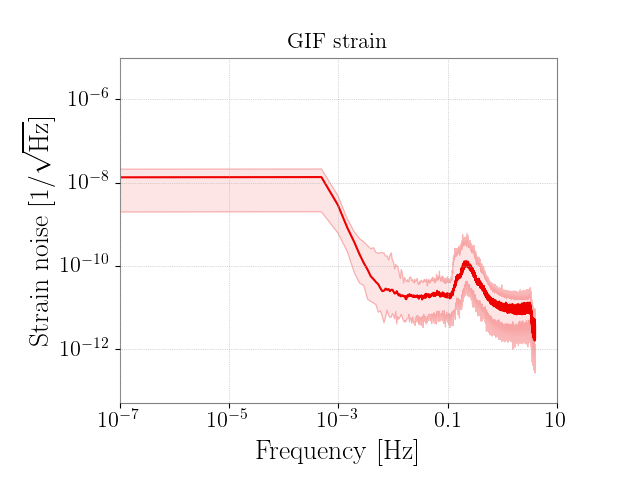
\includegraphics[width=12cm]{./cmrr/asd.png}
  \end{center}
  \caption{Xエンドとセンターエリアにおいた地震計のXアーム方向のASD。エラーバーは95%の有意水準。0.1Hz-0.5Hzの帯域では振幅の大きさが同じである。}\label{img:img1}
\end{figure}
\begin{figure}[h]
  \begin{center}
    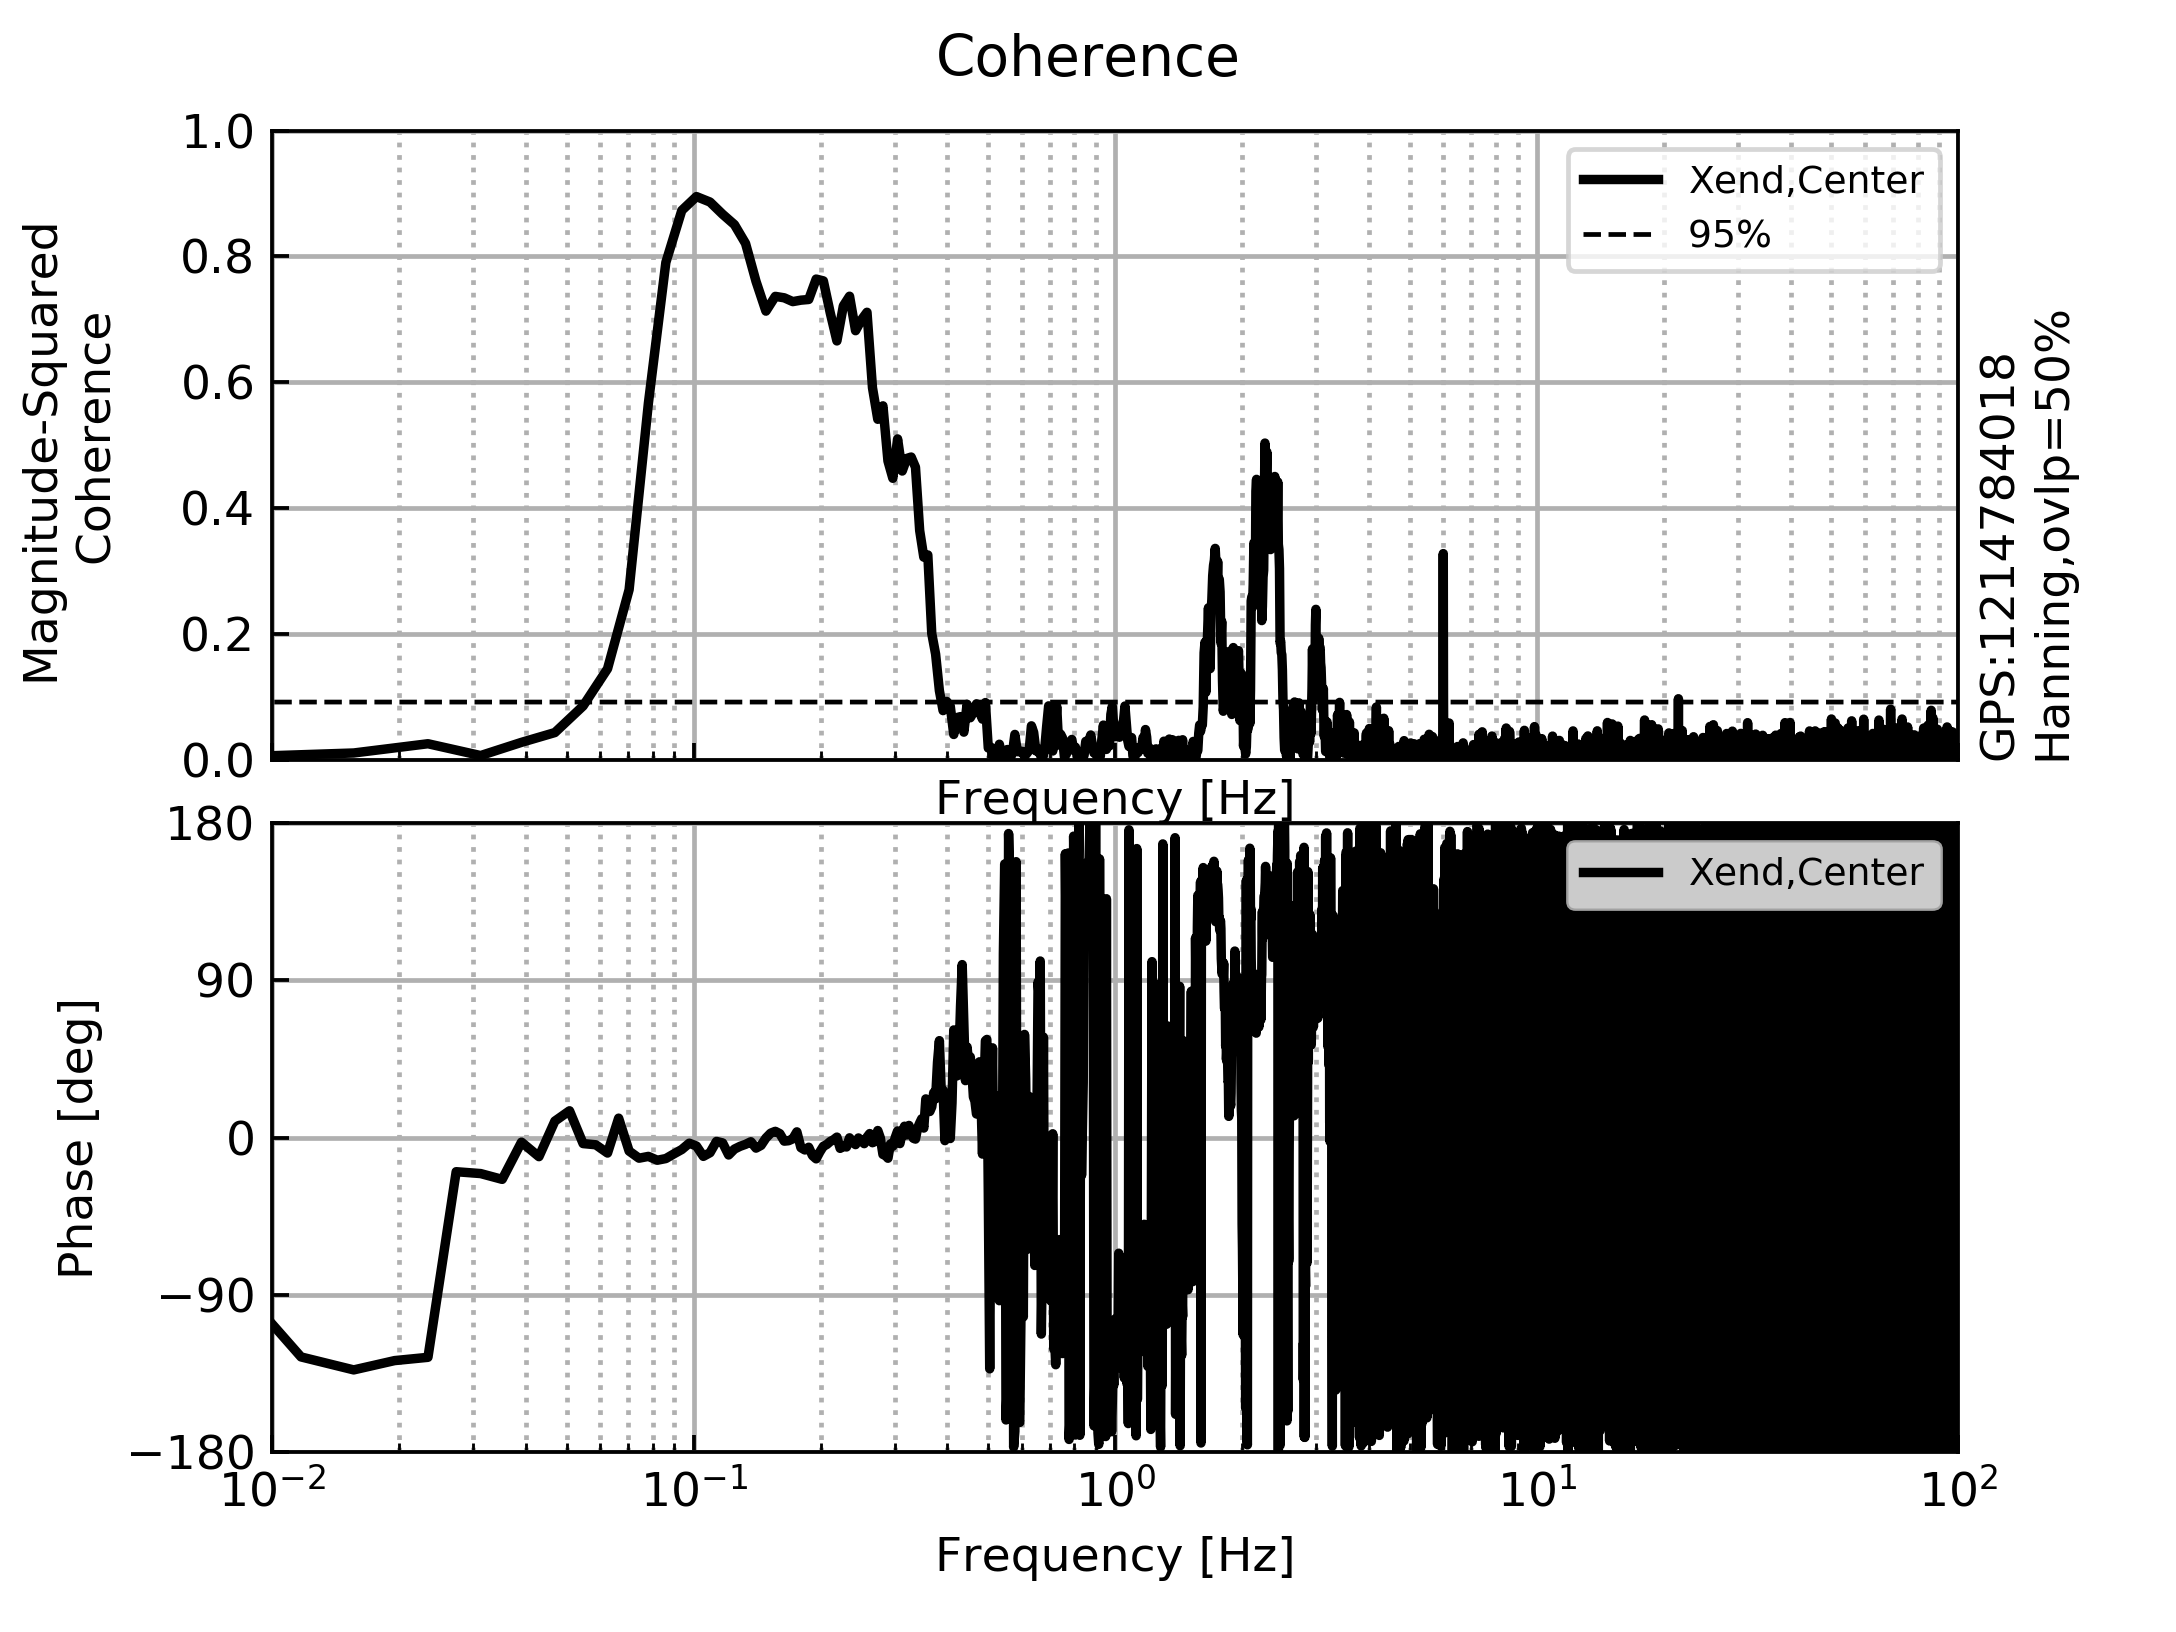
\includegraphics[width=12cm]{./cmrr/coh_seismo.png}
  \end{center}
  \caption{Xエンドとセンターエリアにおいた地震計のXアーム方向同士のコヒーレンス。破線は95%の有意水準でコヒーレンスがゼロであるという帰無仮説。すなわちこれ以上では有意にコヒーレンスがあると言える。0.1-0.3Hzと2Hz付近にコヒーレンスがある。前者は脈動,後者は不明。}\label{img:img2}
\end{figure}


図\ref{img:img2}に,Xエンドとセンターの地震計同士のコヒーレンスを示す。コヒーレンスは0.2Hz付近で有意な値をもち、位相が0度であるため,2点が同相で動いていることを意味している。脈動の帯域では,同相成分のほうが逆相成分よりも大きいことを示唆する。


\subsubsection{平面波モデル($\mathrm{CDMR_{seis}}$)}
実測したデータと比較をするために、Xアームに沿って平面波が伝搬している場合のCDMRを求める。まず変位場$u(x,t)$は、角周波数$\omega$と波数$k$を用いて、
\begin{equation}
  u(x,t) = e^{i(\omega{t}-k{x})}
\end{equation}
となるため,距離$L$離れた二点の逆相成分$u_{\mathrm{diff}}(x,t)$は
\begin{eqnarray}
  u_{\mathrm{diff}}(x,t) &=& \frac{1}{\sqrt{2}}\left( e^{i(\omega{t}-k{x_1})} -e^{i(\omega{t}-k{x_1+L})} \right)\\
  &=& \frac{1}{\sqrt{2}}u(x_1,t)\left( 1-e^{ikL)}  \right)\\
  &=& u(x_1,t)\times{\sqrt{2}{i}}e^{i\frac{kL}{2}}\mathrm{sin}(\frac{kL}{2})
\end{eqnarray}
となる。同相成分$u_\mathrm{com}(x,t)$も同様の計算をして,
\begin{equation}
  u_{\mathrm{com}}(x,t) = u(x_1,t)\times{\sqrt{2}}e^{i\frac{kL}{2}}\mathrm{cos}(\frac{kL}{2})
\end{equation}
となるので,平面波が通過しているときのXアームの$\mathrm{CDMR}$は
\begin{equation}
  \boxed{\mathrm{CDMR_{seis}} = \left| \frac{u(x_1,t)\times{\sqrt{2}}e^{i\frac{kL}{2}}\mathrm{cos}(\frac{kL}{2})}{u(x_1,t)\times{\sqrt{2}{i}}e^{i\frac{kL}{2}}\mathrm{sin}(\frac{kL}{2})}  \right| = \frac{1}{\mathrm{tan\left( \frac{\omega{L}}{2c}  \right)}}}
  \label{eq:eq18}
\end{equation}
で表すことができる。ここで,平面波の分散関係$c=\omega/k$を用いた。


式\ref{eq:eq18}にP波の位相速度$5500\, \mathrm{m/s}$を代入した\footnote[3]{レイリー波だとおもうけど,とりあえずP波の位相速度で考えておく。}ものを図\ref{img:img3}の下図に緑色の破線で示す。0.5Hz以下では低周波になればなるほどCDMRは大きくなる傾向がある。これは,弾性波の波長は0.5Hzでおよそ$3\,\mathrm{km}$の基線長と同程度であったのが,さらに低周波では波長が十分に長くなるので,3km離れた2点はほとんど同相で動きあうことからも理解できる。


この平面波のモデルと、実測データからもとめたCDMRを比較すると、コヒーレンスがある帯域で一致することがわかる。その他の帯域では,ADCノイズや傾斜ノイズによってコヒーレンスがなくなっているため,式\ref{eq:eq33}より,CDMRは1となる。(図\ref{img:img3}下図の青色破線)。


\begin{figure}[htbp]
  \begin{center}
    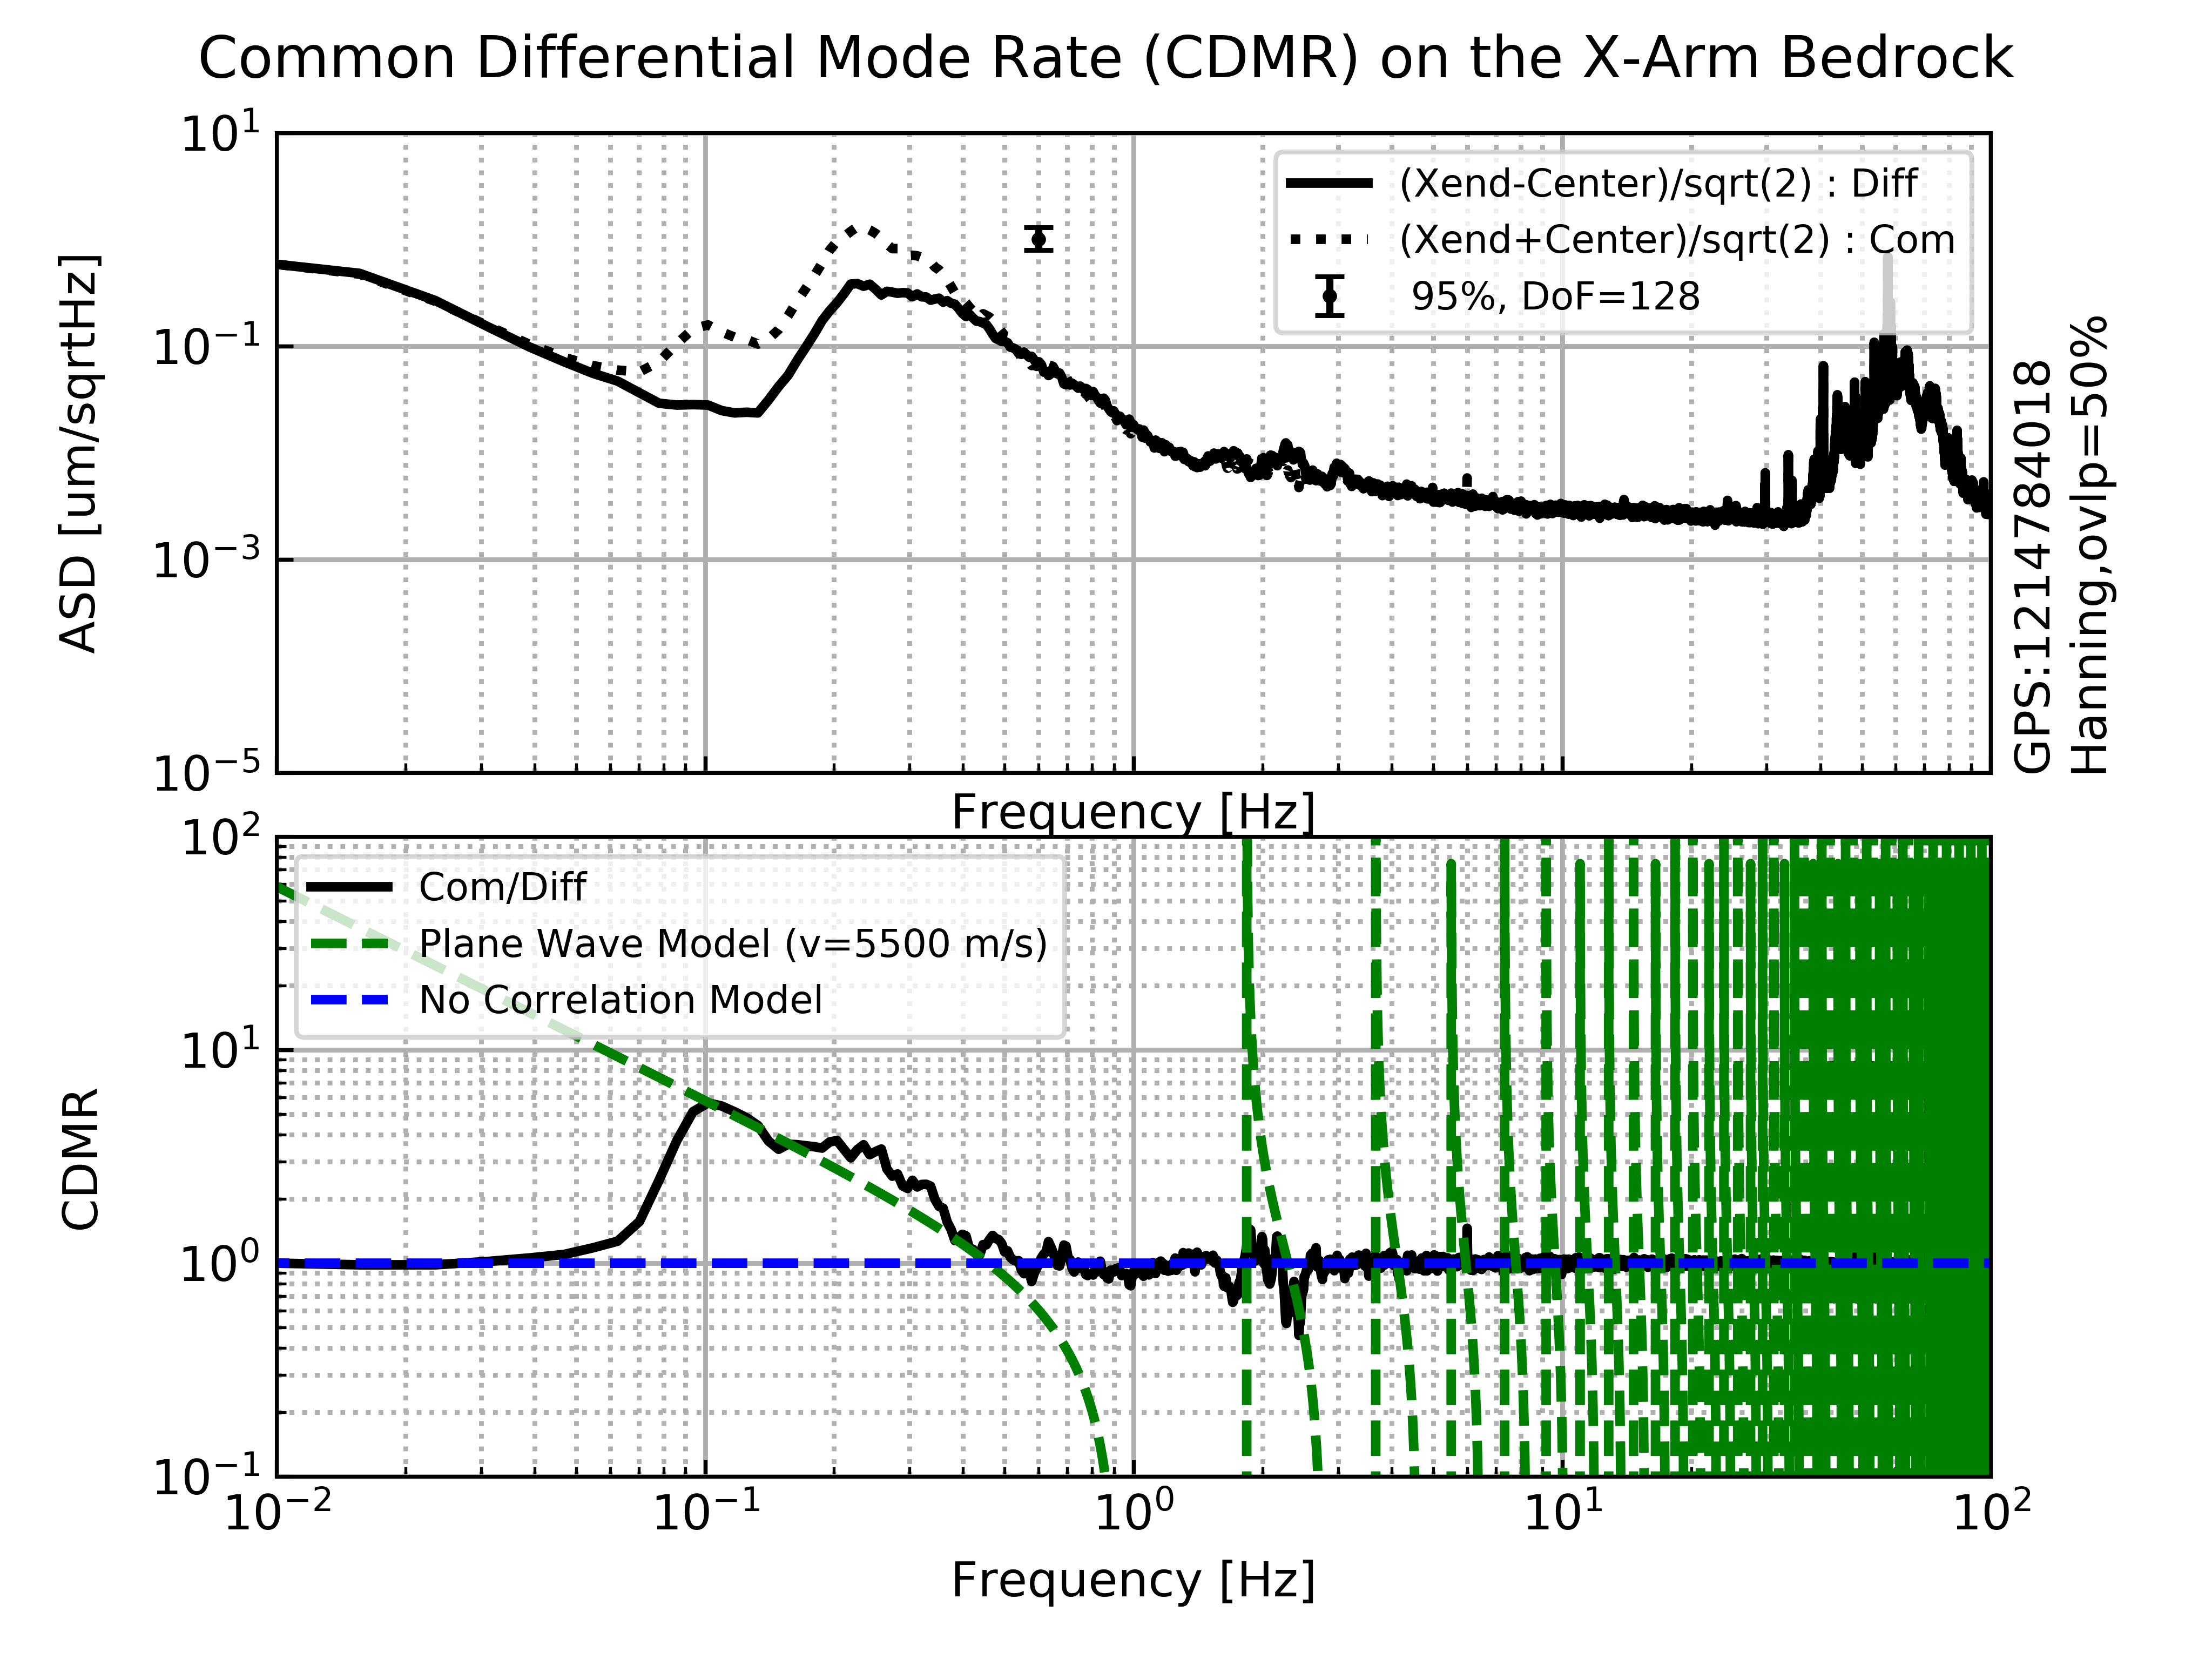
\includegraphics[width=12cm]{./cmrr/cmrr_xarm.png}
  \end{center}
  \caption{上図:3km離れた二点の地面振動の同相成分と逆相成分のASD。0.1-0.2Hz付近にピークをもつ脈動では同相成分のほうが逆相成分よりも大きい。下図:同相成分と逆相成分の比(CDMR)。緑色の破線は,位相速度$5500\, \mathrm{m/s}$平面波がXアームを伝搬した場合のCDMRを示す。青色の破線は,相関がない場合のCMDRを示す。脈動はコヒーレンスがあり,波長はKAGRAの基線長よりも長いので,同相雑音が低減されている。}\label{img:img3}
\end{figure}


\subsubsection{平面波モデル($\mathrm{CDMR_{gif}}$)}
次に、GIFと地震計の比較のために、式\ref{eq:eq23}の逆相成分をGIFのひずみ計で置き換えた$\mathrm{CDMR_{gif}}$を計算する。GIFのひずみ計は1500m離れた2点間のひずみ$\varepsilon_{\mathrm{gif}}$を測っている。そのため,3km離れた二点の地面振動の逆相成分$x_{\mathrm{diff_{gif}}}$は,
\begin{equation}
  x_{\mathrm{diff_{gif}}} = \varepsilon_{\mathrm{gif}}\times \frac{3000}{\sqrt{2}}\label{eq:eq34} 
\end{equation}
と表すことができる。\footnote[5]{数kmスケールの基線長のひずみ応答は数Hzまで平坦なので,脈動以下の周波数帯域では,単純にスケール倍すればいい。}


平面波が伝搬しているとき,速度$v(x,t)$は$v(x,t) \equiv \frac{\partial{u}}{\partial{t}} = i\omega{u(x,t)}$であり、ひずみ$\epsilon(x,t) $ は$\epsilon(x,t) \equiv \frac{\partial{u}}{\partial{x}} = -ik{u(x,t)}$となるので、両者の振幅比は

\begin{equation}
  \left| \frac{A_v}{A_\epsilon} \right|= c \label{eq:eq40}
\end{equation}
となって,位相速度$c$で表すことができる。


さて,GIFで逆相成分を置き換えた$\mathrm{CDMR_{gif}}$は、式\ref{eq:eq36}と式\ref{eq:eq34}をもちいて、
\begin{empheq}[box=\fbox]{align}
  CDMR_{\mathrm{gif}} &= \frac{A_{\mathrm{x}}\sqrt{\left(1+\Re[coh]\right)}}{{A_{\epsilon}L}/{\sqrt{2}}}  \label{eq:eq37} \\
  &= \sqrt{2\left(1+\Re[coh]\right)}\frac{A_{v}}{A_{\epsilon}}\frac{\omega}{L}\label{eq:eq38} \\
  &= \sqrt{2\left(1+\Re[coh]\right)}\frac{\omega{c}}{L} \label{eq:eq39} \\
\end{empheq}
となる。\ref{eq:eq38}式から\ref{eq:eq39}式へは、速度とひずみの関係式\ref{eq:eq40}をもちいた。


式(\ref{eq:eq39})の位相速度に花崗岩の弾性波速度である5500m/sを代入して図\ref{img:img3}の下図に赤色の破線で示す。地震計と同様に脈動の帯域では平面波のモデルと一致する。それより高周波ではGIFは周波数ノイズに埋もれて地震計の同相成分よりも大きいので,CDMRは平面波のモデルよりも小さくなっている。一方で脈動より低周波では,GIFは基線長伸縮をみているがそれに対応する地震計の逆相成分は,GIFよりも大きい。この帯域では,図\ref{img:img3}で示したように,CDMRが1であったため,地震計同士が無相関で動いている。つまり,傾斜などのローカルなノイズをみていて,基線長伸縮をみていないことがわかる。

\begin{figure}[htbp]
  \begin{center}
    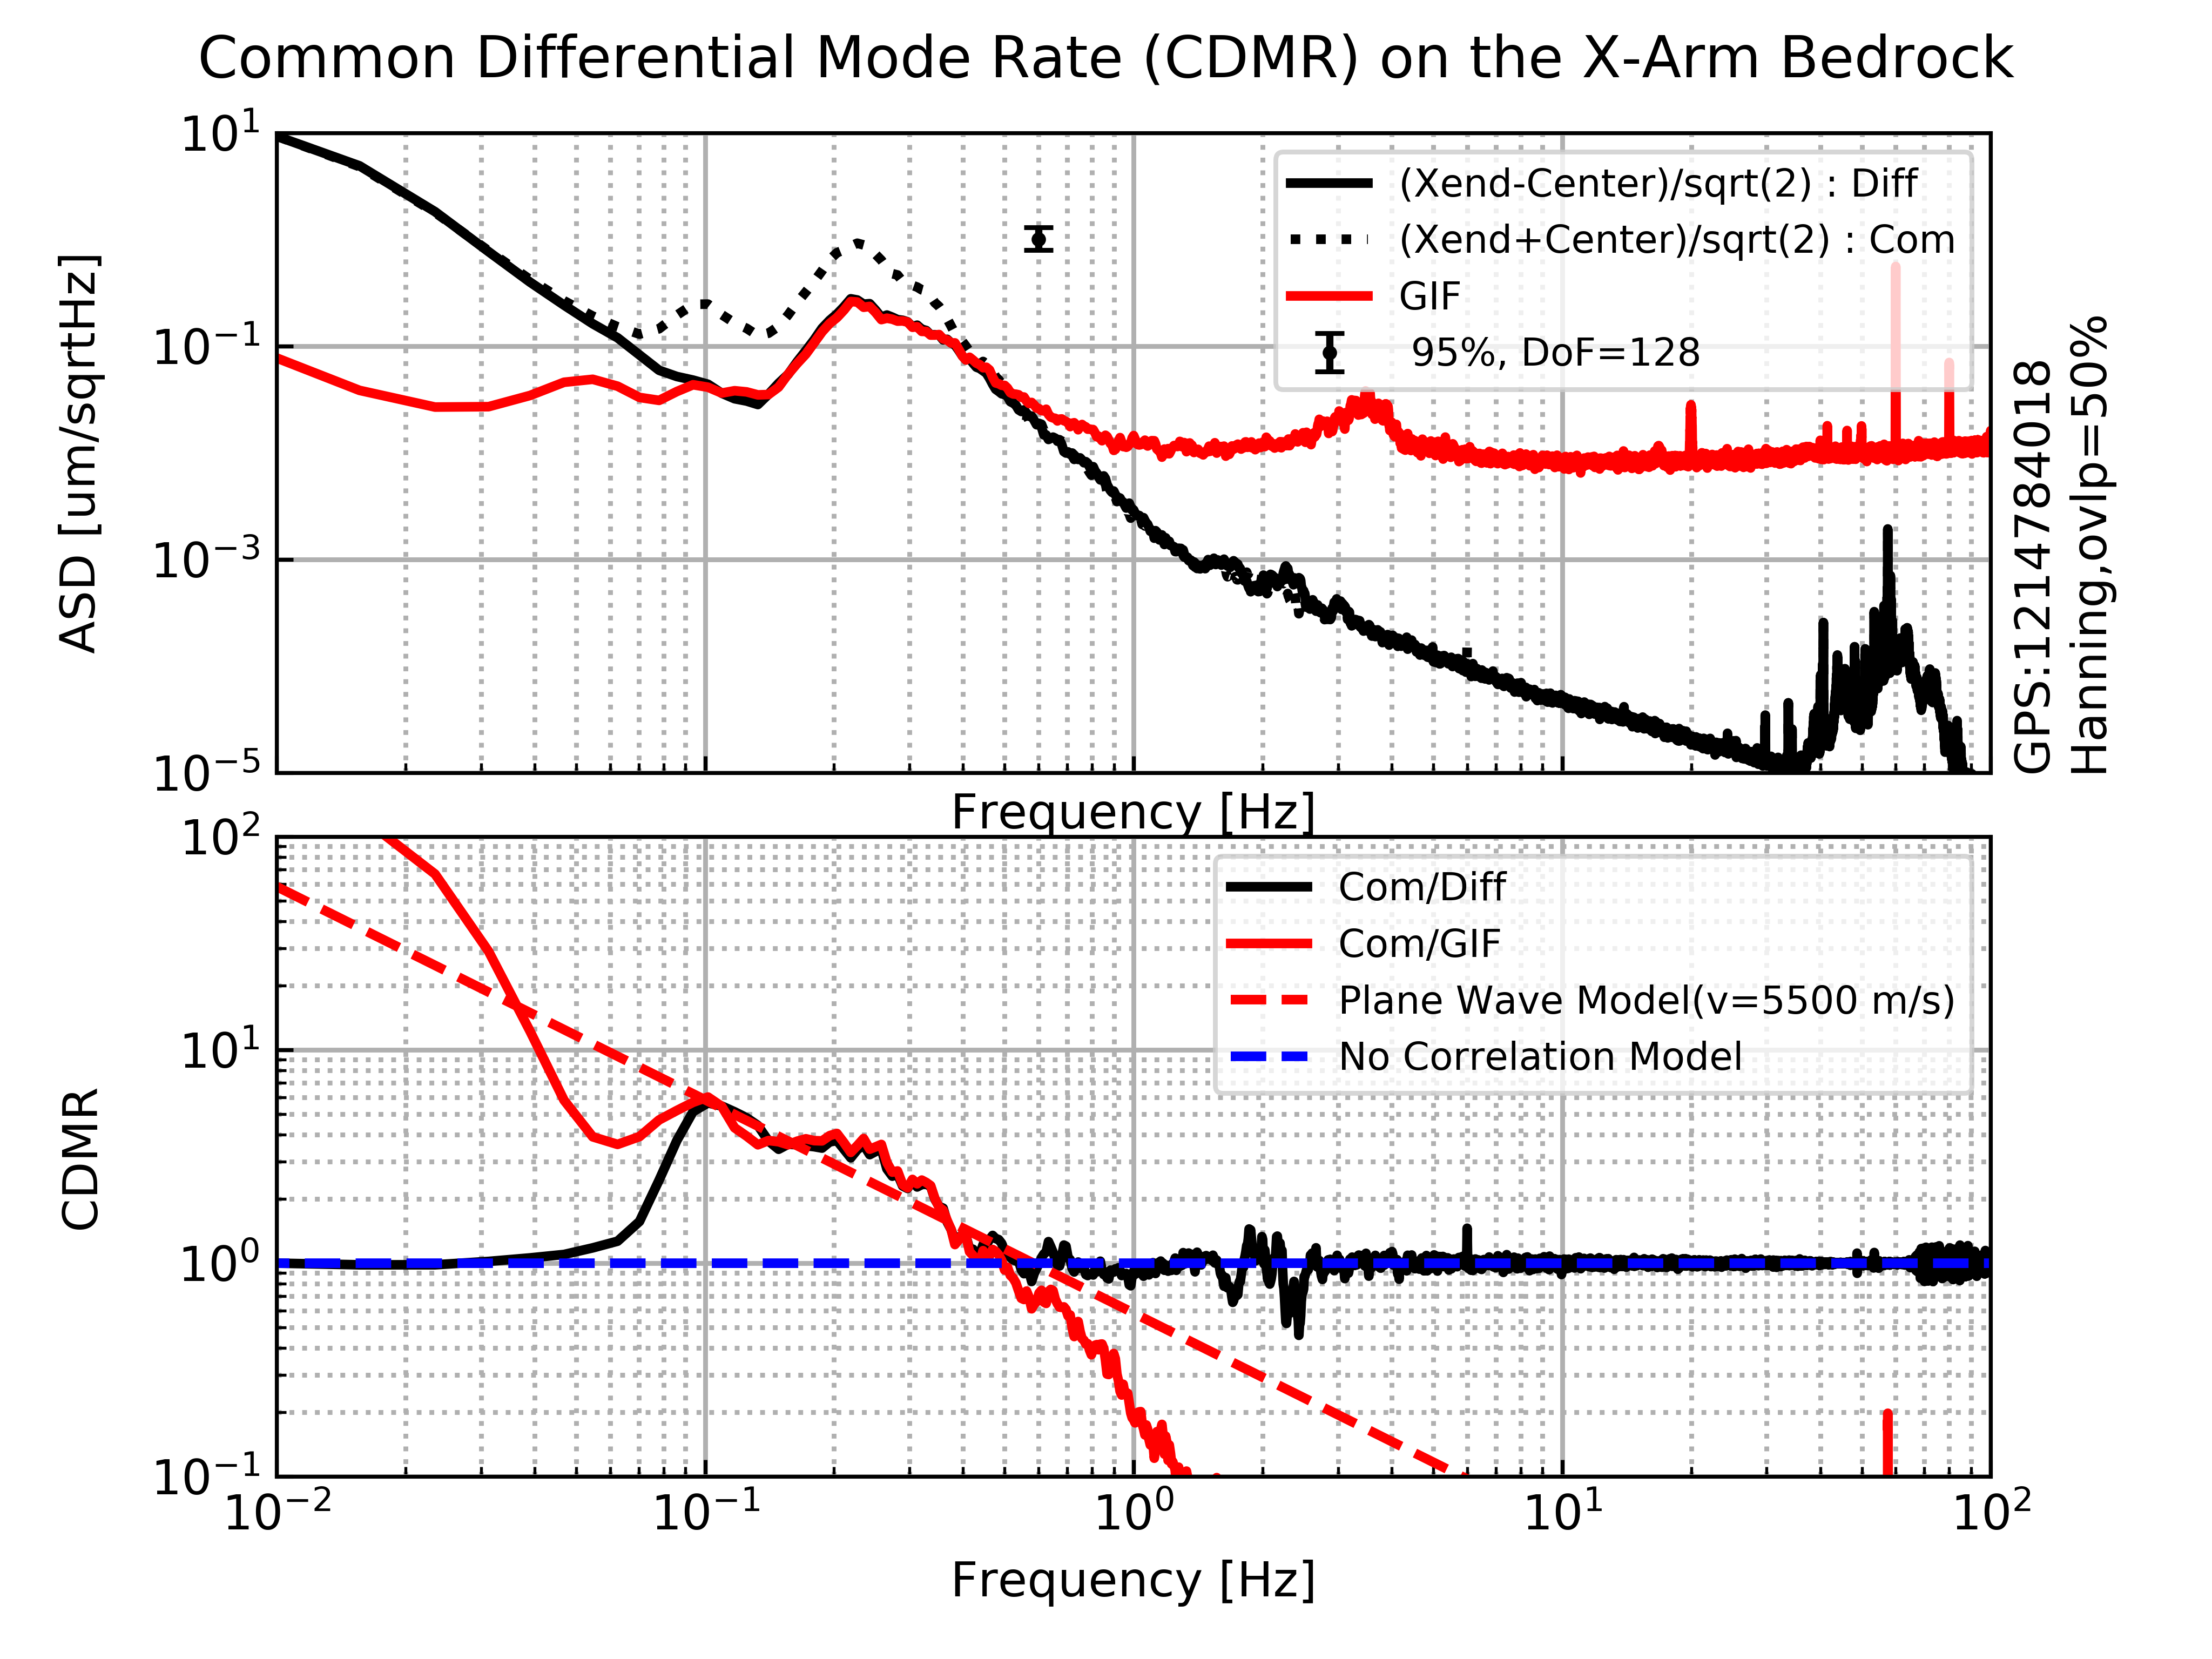
\includegraphics[width=12cm]{./cmrr/cmrr_xarm_gif.png}
  \end{center}
  \caption{図\ref{img:img3}にGIFで推定した逆相成分を加えて比較。上図:同相成分と逆相成分の比較。GIFで推定した逆相成分は,脈動の帯域では地震計でもとめたものと一致しているが,低周波では一致しない。これは,図\ref{img:img3}のこの帯域で,CDMRが1で2つの地震計が無相関だったことからも,地震計がローカルなノイズをみていることがわかる。そのためGIFは地震計よりも低周波で感度をもつことが確認できる。下図:逆相成分をGIFで推定したものを加えて比較。式\ref{eq:eq}で表される平面波モデル(赤線の破線)は,図\ref{img:img3}と同様に,脈動の帯域で実測値と一致する。その他の帯域では,先に述べたように,高周波はGIFがADCノイズで,低周波は地震計が傾きノイズをみているため,モデルとは一致しない。
  }\label{img:img4}
\end{figure}


\subsection{長期データ}
長期間の基線長伸縮スペクトルをここでのべる。今後KAGRAの基線長伸縮として引用できるようなもの。一年をとおしてデータを解析してみる。平均的なスペクトルを知りたいので地震や台風のときは除く、もしくは「うるさいとき」という感じで、スペクトルを乗せる。


\subsection{まとめ}
本章では、同相成分と逆相成分の比であるCommon Differential Mode Ratio (CDMR)という量を定義して、Xアームを平面波が通過している簡単なモデルと、実測データを比較した。その結果、脈動ではセンターとXエンド同士で有意なコヒーレンスがあった。この帯域では、平面波のモデルと実測データが一致し、2点は同相で動いていることがわかった。そして、CDMRを計算すると、最大で逆相成分が同相成分の1/4になっており、3kmの基線長でも逆相成分の低減が確認できた。


また、地震計とひずみ計の比較もおこなった。

ひずみ計は1500mの基線長伸縮を直接みており、地震計とは異なって、原理的には地面の傾斜成分は並進方向にカップルしないため、低周波


\section{環境変動によるXアームの基線長伸縮}
波浪や地震、気圧・水圧などの環境変化によって基線長伸縮がどう影響をうけるか述べる。

\subsection{波浪}
\subsection{地震}
\subsection{気圧}
\subsection{水圧}


